%% Author_tex.tex
%% V1.0
%% 2012/13/12
%% developed by Techset
%%
%% This file describes the coding for rsproca.cls

\documentclass[]{rsos}%%%%where rsos is the template name

\usepackage{amsmath}
\usepackage{amssymb}
\usepackage{amsfonts}
\usepackage{amsthm}
\usepackage{graphicx}
\usepackage{endfloat}
\usepackage{endnotes}

\usepackage{verbatim}
\usepackage{times}
\usepackage{helvet}
\usepackage{courier}
\usepackage{bm}
\usepackage{url}
\usepackage[english]{babel}
\usepackage{dcolumn}

\usepackage[mathlines]{lineno}

\usepackage[activate={true,nocompatibility},final,tracking=true,kerning=true,spacing=true,factor=1100,stretch=10,shrink=10]{microtype}
\microtypecontext{spacing=nonfrench}
\usepackage{setspace}
\usepackage{epigraph}

\usepackage[numbers]{natbib}
\bibliographystyle{rspublicnat}

\jname{rsos}
\Journal{R Soc Open Science}
%%%% *** Do not adjust lengths that control margins, column widths, etc. ***

%%%%%%%%%%% Defining Enunciations  %%%%%%%%%%%
\newtheorem{theorem}{\bf Theorem}[section]
\newtheorem{condition}{\bf Condition}[section]
\newtheorem{corollary}{\bf Corollary}[section]
%%%%%%%%%%%%%%%%%%%%%%%%%%%%%%%%%%%%%%%%%%%%%%%


\begin{document}

%%%% Article title to be placed here
\title{Important and Unique and Central: Species' Relevance in Food Webs}

\author{%%%% Author details
G. V. Dalla Riva$^{1}$ and Carey E. Priebe$^{2}$}

%%%%%%%%% Insert author address here
\address{$^{1}$Biomathematics Research Centre\\ School of Mathematics and Statistics\\ University of Canterbury\\ Christchurch, New Zealand\\
$^{2}$Department of Applied Mathematics and Statistics\\ Whiting School of Engineering\\ Johns Hopkins University\\ Baltimore, MD}

%%%% Subject entries to be placed here %%%%
\subject{Ecology, Evolution, Mathematical Modelling}

%%%% Keyword entries to be placed here %%%%
\keywords{Food Webs, Centrality, Functional Diversity, Evolutionary Distinctiveness, Random Graphs, Keystone Species}

%%%% Insert corresponding author and its email address}
\corres{Giulio Valentino Dalla Riva\\
\email{gvd16@uclive.ac.nz}}

%%%% Abstract text to be placed here %%%%%%%%%%%%
\begin{abstract}
Estimating the species' relative importance in an ecosystem  is a crucial task at the
core of all scientifically informed efforts to preserve the planet's biodiversity.
Unfortunately, the species' diversity makes
it hard to identify traits with a functional role across a large ecosystem.
Therefore, researchers have adopted a graph description of trophic interactions
in terms of food webs and graph-theoretical measures have been proposed to
estimate species' importance. However, these measures are often derived from
rigid models and their applicability to food webs, which are characterized by
stochastic behaviours, can be limited. Here, we compute the position of the species
in the (abstract) functional trait space of their food web and estimate the species' relative
importance for the food web's stability, their contribution to the food web's
functional diversity and their ecological uniqueness. We compare
the species' relevance as determined by our novel measures and six classic
measures, showing a general agreement of local and global measures: central species
tend to be ecologically original. Next, we simulate interaction weights and show that our
measures are robust: the set of species identified as highly unique using only topological
data is preserved when interaction weights are accounted for.  Finally, we explore the phylogenetic distribution of
the species' relevance in the Serengeti National Park food web and identify a clade
that is both ecologically and evolutionary distinctive, although there is no linear correlation
between the two distinctiveness.
\end{abstract}
%%%%%%%%%%%%%%%%%%%%%%%%%%%

%%%%%%%%%% Insert the texts which can accomdate on firstpage in the tag "fmtext" %%%%%


%%%%%%%%%%%%%%% End of first page %%%%%%%%%%%%%%%%%%%%%

\maketitle



\epigraph{I go for all, because someone must go for all.}{\emph{The Brothers Karamazov}\\ \textbf{Fyodor Dostoyevsky} \\ Translated by Constance Garnett}


\section{Introduction}\label{sec:intro}

The need for scientifically informed conservation policies boosted the attempts
to estimate species' relative importance in food webs: the graphs describing
the flows of energy between species in an ecosystem \citep{may2009food}. A
sound approach to assess a species' contribution to an ecosystem is based on the
concept of functional diversity. As summarised by \citet*[pg. 742]{petchey2006functional},
\begin{quote}
[$\dots$] measuring functional diversity is about measuring functional traits diversity, where functional traits are components
of an organism's phenotype that influence ecosystem level processes.
\end{quote}
In this context, the contribution of a species to the functional diversity of a food
web is captured by the traits diversity loss that we would observe after the removal
of that species \citep{villeger2008new, fontana2015individual}. However,
identifying suitable phenotypic traits and collecting all the necessary
data across a full food web is often ambitious. The tangled intricacy of food
webs, where there are often thousands of interactions between hundreds of plants and
animals, motivates the use of complex-network tools for solving ecological problems
\citep{proulx2005network}. Centrality measures---graph theoretical measures
developed in economic, social, technological and theoretical scenarios to
identify crucial nodes in a network \citep{newman2009networks}---have been
proposed to assess a species' centrality and to identify the species that play a
crucial role within an ecosystem
\citep{estrada2007characterization,lai2012centrality}.

The evolutionary distinctiveness of species (i.e., the amount of
\emph{exclusive} evolutionary information hinging on a species) is an
intrinsic component of biodiversity \citep{mace2003preserving} and the
evolutionary diversity of species is used as a proxy for a species' functional
diversity \citep{winter2013phylogenetic}. Evolutionary diversity has been shown
to promote ecosystem stability \citep{cadotte2012phylogenetic}. Accordingly, it
has been argued that the evolutionary distinctiveness of species should be one
of the factors grounding conservation efforts
\citep{faith1992conservation,redding2006incorporating,isaac2007mammals}.
However, the exact relationship between the evolutionary and food-web
distinctiveness of a species is an open problem
\citep{gerhold2015phylogenetic,miranda2015congruence}.

In \citep{dallariva2015exploring} we introduced directed RDPG for food webs: from
the classic binary description of a food web---its adjacency matrix---we
estimate species' position in an \emph{abstract functional trait} metric space
so that the species' interaction probabilities are determined by the pairwise
distance structure: the probability of observing an interaction from species $i$
to species $j$ (e.g., $j$ feeding on $i$) is given by the dot product of the vulnerability
functional traits of $i$ and the foraging functional traits of $j$.

This motivates the distinction between a food web's backbone---its most statistically persistent
structure---and its fine wiring, which is more sensitive to contingent ecological
factors or stochastic noise \citep{grady2012robust, bellingeri2015food}. A robust ordering of species
based on their ecological relevance should not be too sensitive on
the fine wiring of a food web \citep{livi2011identifying}.

Here, we show how the abstract functional trait space, estimated by the RDPG model,
offers a unified framework in which to assess species' importance, uniqueness
and diversity. We propose three measures, relying only on topological food-web data,
which can serve as proxies for measures based on phenotypic data. 

Building on the existing measures of trophic similarity
\citep{yodzis1999search,luczkovich2003defining,jordan2009trophic}, we will define
the \emph{uniqueness} of a species' food-web role  as its
isolation (i.e., the average distance to all the other species) in the abstract
functional traits space estimated by the RDPG model. To measure the 
species' relative importance in a food web, we define a species' \emph{strain} as the
effect that removing that species has on the estimated abstract functional
trait space: for each focal species in the food web we measure the total
distance between the remaining species' positions in the abstract functional
trait space before and after the removal of the focal species. The strain of a species
captures a global effect at the whole food-web scale, rather than a local property of its interactions structure.
Borrowing from the functional diversity literature, we estimate the functional diversity of a food web as the
volume of the convex hull enclosing all the species' abstract functional
traits. Accordingly, we define the contribution of a species to the functional
diversity of a food web as the loss in diversity caused by the removal of that
species.  Focussing on the vulnerability, on the foraging or both the
vulnerability and foraging abstract functional traits, we can assess a
species' relevance as prey, as a predator or as both predator and prey. We
distinguish among the species' strain, uniqueness, and contribution to the
functional diversity as prey (\emph{outward} strain, uniqueness, and contribution to
the functional diversity), as a predator (\emph{inward} strain, uniqueness,
and contribution to the functional diversity) or as both a predator and prey
(\emph{total} strain, uniqueness, and contribution to the functional diversity).

We correlate these novel measures among each other as well as with six classic
network centrality measures, and we explore their distribution among the clades
present in the food web. In particular, we test whether the distribution of
ecological relevance among the tips of the Serengeti National Park food web's
phylogeny is compatible with an evolutionary model of traits evolution.
Finally, we examine the hypothesis that the species' ecological relevance and
evolutionary distinctiveness are indeed correlated.


%%%%%%%%%%%%%%%%%%%%%%%%%%%%%%
%%%%%%%%%% METHODS %%%%%%%%%%%%%%
%%%%%%%%%%%%%%%%%%%%%%%%%%%%%%

\section{Data and methods}
% 
 \subsection{Food webs and phylogenies}
 We focus our analysis on the Serengeti National Park food web as published
 by \citet{baskerville2011spatial}. We present the result of the analysis for a binary
 (unweighted) version of the web. It is a large food web with 129
 plants, 23 herbivores and 9 carnivores. Most of the links (507 out of 590) are between
 herbivores and plants. The food web is less densely connected than other food webs, which is a
 consequence of the higher than the usual taxonomic resolution of plants. To
 test the general applicability of our framework, we
 summarise the results for other three large food webs:
 an independent compilation of the Serengeti National Park food web
 \citep{de2011serengeti} and two marine food webs, one for the Caribbean Sea
 \citep{opitz1996trophic} and one for the Antarctic Weddell Sea
 \citep{jennings2002long}. The dated phylogenetic tree (available on-line) for
 the species in the two Serengeti food webs has been compiled from molecular
 data by De Zwaan \emph{et al.}. We approximated the real phylogeny for the
 other webs via a cladogram obtained from the species' taxonomy as given by the
 Integrated Taxonomic Information System (http://www.itis.gov; information retrieved on 11 November 2014).

\subsection{Random dot product graphs}\label{subsec:method_rdpg}

Let $A$ be a food web including $S$ species.
Given a model dimension $d$, under the RDPG model, each species $i$ in $A$
is associated to a pair of abstract functional trait vectors of dimension $d$.
The two vectors are the \emph{rank}-$d$ \emph{vulnerability} traits (or outward traits), which describes the
species as a prey or a resource, and the \emph{rank}-$d$ \emph{foraging} traits (or inward
traits), which describes the species as a predator or a consumer. The probability of observing an
interaction from species $i$ to species $j$ is given by the dot product of the
out traits of $i$ and the in traits of $j$. In other words, the probability of an interaction from $i$ to
$j$ increases as the vulnerability traits of $i$ becomes more similar to the foraging traits of species $j$.
Eventually, if the vulnerability traits of $i$ are identical to the foraging traits of $j$ the probability of an
interaction is one. Conversely, the probability of interaction is zerowhenever the two trait vectors are
orthogonal. Species having similar foraging traits have a similar diet; species having similar vulnerability
traits are in the diet of similar species, see Figure~(\ref{fig:RDPGvignette}).



\begin{figure}[hbt]
 \centering
 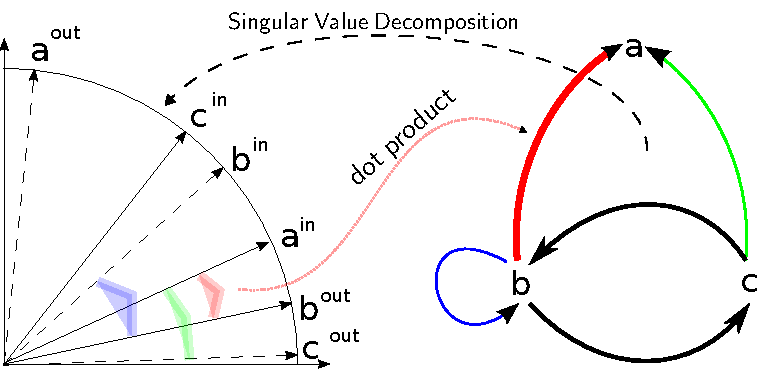
\includegraphics[width=\textwidth]{./images/chap_2/RDPGmodel.pdf}
 \caption{Three hypothetical species represented in a simple (total) functional trait space
(i.e., the overlaying of the vulnerability and foraging trait spaces) and a likely
food web realization under the RDPG model. For each pair of species, we draw the link between them
with a width which is roughly inversely proportional to the angle between the corresponding foraging
and vulnerability functional trait vectors (i.e., directly proportional to their dot product).
Larger dot products correspond to higher interaction probabilities. Conversely, a scaled, truncated, singular
value decomposition of the adjacency matrix of the food web allows us to estimate the position of the species
in the functional trait spaces.}\label{fig:RDPGvignette}
\end{figure}

For an observed food web $A$, the species' traits are estimated through a singular value decomposition
of the adjacency matrix of $A$ after scaling and truncation (see the Supplementary Material for more details). 
The task of identifying a suitable range for the model's dimension is akin to a
dimensionality reduction problem, discussed for the Principal Component
Analysis scenario in \citet{jolliffe2002principal}. This can be solved
through the examination of the sequence of singular values of the adjacency matrix
of $A$.

\subsection{Food-web relevance}

\subsubsection{Strain}
The strain of species $i$ measures the effect that the removal of $i$ from the food web
has on the remaining species' abstract functional traits, as estimated from the
RDPG model. The effect is measured for species either as predators, as prey or as both. 
Let $X(A)$ be the matrix of either the inward, outward or total rank-$d$ abstract
functional traits (the last one being the matrix in  which the first $d$ columns are
given by the inward traits and the next $d$ columns are given by the outward traits).
We let $X(A)^{r(i)}$ denote the matrix of the (inward, outward or total)
functional traits for all the species in the food web $A$ except $i$ (i.e.,
the matrix obtained by $X(A)$ removing the $i$th row). Moreover, we let
$X\left(A^{d(i)}\right)$ denote the matrix of traits for the species in the food
web $A$ that has been computed after having dropped the species $i$ from the food web with
all its interactions (i.e., the matrix of traits computed after removing the $i$th row and column from $A$).
Both $X(A)^{r(i)}$ and $X\left(A^{d(i)}\right)$ are matrices with $S-1$ species (each species
in $A$ but $i$) and $d$ columns (the model's dimension). In $X(A)^{r(i)}$, the functional
traits are computed before removing $i$, in $X\left(A^{d(i)}\right)$ they are computed
after the removal event.

The parameter matrix of an RDPG model is defined up to an orthogonal transformation
\citep{dallariva2015exploring}. Therefore, the distance between
$X(A)^{r(i)}$ and $X\left(A^{d(i)}\right)$ is determined by both the species
removal effect and, possibly, the change of basis for the RDPG parameters.
Thus, we defined the (inward, outward or total) rank-$d$ strain of the species $i$ as
the Procrustes distance \citep{dryden1998statistical} between $X(A)^{r(i)}$ and $X\left(A^{d(i)}\right)$
(i.e., the minimum distance between $X(A)^{r(i)}$ and an orthogonal transformation of $X\left(A^{d(i)}\right)$).

We are interested in the use of RDPG-based measures to value species in a way that
is robust to model parameters. Therefore, we tested whether the species' ordering by strain
was sensitive to the choice of model dimensionality and performed a pairwise correlation test for each pair of
dimensions in the range $\left[1, \dots, 15 \right]$. Notice that the latter upper
range limit is much greater than the suitable upper bound for model dimensionality found
in \citep{dallariva2015exploring}.

\subsubsection{Uniqueness}
We define the rank-$d$ \emph{uniqueness} of a species in a food web, either as
a predator, prey or both, as the average of its
Euclidean distance to every other species in the $d$-dimensional (inward, outward or total)
abstract functional trait space.

Let \(d\left(p,q\right)\) denote the \(d\) dimensional Euclidean
distance between the point \(p\) and \(q\); let
\(\langle f(i,j) \rangle_j\) be the mean of the function \(f\) over all
the species \(j\) except \(i\). That is,
\(\langle f(i,j) \rangle_j = \frac{1}{S}\sum_{j \neq i}(f(i,j))\). Then,
the \textbf{uniqueness} of species \(i\) is defined as:
\begin{equation}
\mbox{uniqueness($i$)} := \langle d\left( X(A)_i,X(A)_j\right)\rangle_j \, .
\end{equation}

The relative uniqueness of the species in a food web is robust to orthogonal
transformations of the food web's abstract functional space:
indeed, the pairwise distance structure is invariant to rotations and
translation, while uniform rescaling leaves unchanged the ordering.

\subsubsection{Diversity}
The volume of the convex hull of a community of species in the traits space is a
proxy for its functional diversity \citep{villeger2008new}. Here, we define the
contribution of species $i$ to a food web's abstract functional diversity as
the difference in volume between the convex hull of the species traits, in the
(inward, outward or total) abstract functional space, before and after species $i$ is removed.

Let $\mathcal{H}^{(d)}\left( X \right)$ be the convex hull of a set of points $X$ in
the real space $\mathbb{R}^d$. Then, we define $V\left(\mathcal{H}^{(d)}\left( X \right) \right)$
its $d$ dimensional volume---or the area of the convex hull of $X$ if $d=2$.
We identify $X(A)$ with the set of points of the species in $A$ and $X(A)^{r(i)}$
with the set of points of the species in $A$ but $i$. Then, the contribution
to the food-web functional diversity of a species $i$ is the difference in volume
between the two convex hulls
\begin{equation}
\mbox{diversity($i$)} := V\left(\mathcal{H}^{(d)}\left( X(A) \right) \right) - V\left(\mathcal{H}^{(d)}\left( X(A)^{r(i)} \right) \right)
\end{equation}
and we define its normalized version as
\begin{equation}
\mbox{normdiversity($i$)} := \frac{V\left(\mathcal{H}^{(d)}\left( X(A) \right) \right) - V\left(\mathcal{H}^{(d)}\left( X(A)^{r(i)} \right) \right)}{V\left(\mathcal{H}^{(d)}\left( X(A) \right) \right)}
\end{equation}

Again, the relative diversity and normalized diversity of a species is robust to
orthogonal transformations of the abstract functional space.

In this sense, all the three RDPG based measures we defined are robust to the non identifiability
of the (inward, outward and total) abstract functional traits.


\subsubsection{Topological centralities}

We assessed the keystone centrality of a species $i$ in a food web $A$ by using
six different (topological) network measures following
\citet{estrada2007characterization}: degree centrality, betweenness centrality \citep{brandes2001faster},
closeness centrality  \citep{freeman1979centrality}, eigenvector centrality
\citep{bonacich2001eigenvector}, information centrality
\citep{stephenson1989rethinking}, subgraph centrality
\citep{estrada2005subgraph} (see \citep{jordan2009trophic} for
more details about their ecological interpretation). We choose these topological
measures as their evaluation does not necessitate morphological trait data nor
interaction weights (see the Supplementary Material for more details about the centrality
measures we considered).

\subsection{Weighted networks}

The main results are presented for binary food webs, expressing the presence or absence
of the interactions. However, the components of the species'
diets are not equally important. To test the extent to which our ecological relevance measures are robust to the specification
of interactions' weights, we compared the ranking of the species based on \emph{strain} and \emph{mean distance} as
computed from topological data with the rankings we obtained by simulating interactions weights.
To do so, we sampled the interactions weights from a Log-Normal distribution,
truncated so that their minimum value was $10^{-6}$ (i.e., assuming that the topological structure
of the observed food web correspond to the real one) and normalised so that the maximum value
was $1$.

\subsection{Phylogenetic diversity}
The concept of ``phylogenetic diversity'' \citep{faith1992conservation,hartmann2007phylogenetic}
constitutes an alternative point of view from which to evaluate the diversity of a
community of species. The phylogenetic diversity of an evolutionary tree is the total sum of branch lengths in that
phylogeny. This concept has been applied in the prioritisation of species
for conservation purposes \citep{faith1992conservation,mace2003preserving}.  We
estimated species' evolutionary distinctiveness by
measuring its fair proportion value \citep{isaac2007mammals}, equal
splits value \citep{redding2006incorporating} and the length of the terminal
phylogenetic branch leading to that species, following \citet{faye2015valuing}.
The fair proportion and equal split scores attempt to apportion the total
evolutionary  history of a phylogeny among the extant species.

\subsection{Comparative analysis}
Because of their shared evolutionary histories, we would expect to observe more similar
traits for more closely related species \citep{cavalli1967phylogenetic,felsenstein1985phylogenies}. 
The evolutionary dependency of species arises the statistical issue of controlling and correcting
for the phylogenetic covariation structure of the observed species' traits.
To select the appropriate evolutionary model, we compute the relative Akaike information criterion
corrected for finite sample size (AICc, see \citet{hurvich1989regression})
of four distinct models \citep{garamszegi2014multimodel}. We
consider an uncorrelated null model, a Brownian motion model
\citep{felsenstein1985phylogenies}, an Ornstein--Uhlenbeck model \citep{hansen1997stabilizing} (i.e.,
a Brownian motion with attraction toward an optimum) and a model with early
burst of differentiation \citep{harmon2010early}.
We test for linear correlations among the (inward, outward and total) novel measures (of strain,
uniqueness, and contribution to functional diversity) and among (inward, outward and total)
strain and uniqueness and the six keystone centralities.

%%%%%%%%%%%%%%%%%%%%%%%%%%%%%%
%%%%%%%%%%  RESULTS  %%%%%%%%%%%%%%
%%%%%%%%%%%%%%%%%%%%%%%%%%%%%%

\section{Results}

We computed the species strain for $d \in \left[ 1, \dots,  15 \right]$ (Figure~(\ref{fig:strain_1}
a)). In \citep{dallariva2015exploring} we estimated a suitable model dimension $d = 3$
for the Serengeti National Park food web.  The species'
strain (model dimension $d = 3$) has an average value of $0.032$ and a variance of $0.017$;
a small number of species have a high strain (Figure~(\ref{fig:strain_1} b)). The
three species with the highest strain are all in the Afrotheria clade (and represent
the totality of that clade in the food web). These are \emph{Procavia
capensis} (rock hyrax, strain $= 1.316$), \emph{Heterohyrax
brucei} (yellow-spotted rock hyrax, strain $= 0.884$) and
\emph{Loxodonta africana} (the African bush elephant, strain
$= 0.317$). The ordering of species based on their strain is robust to the
choice of model dimension, in the range $d \in \left[ 1, \dots,  15 \right]$
(Figure~(\ref{fig:strain_1} c)). Every pairwise ordering correlation in the analysed
interval is significant at $p < 0.01$ (this result is also confirmed
by the analysis of the independent assembly of the Serengeti National Park food
web by \cite{de2011serengeti}).

\begin{figure}[hbt]
 \centering
 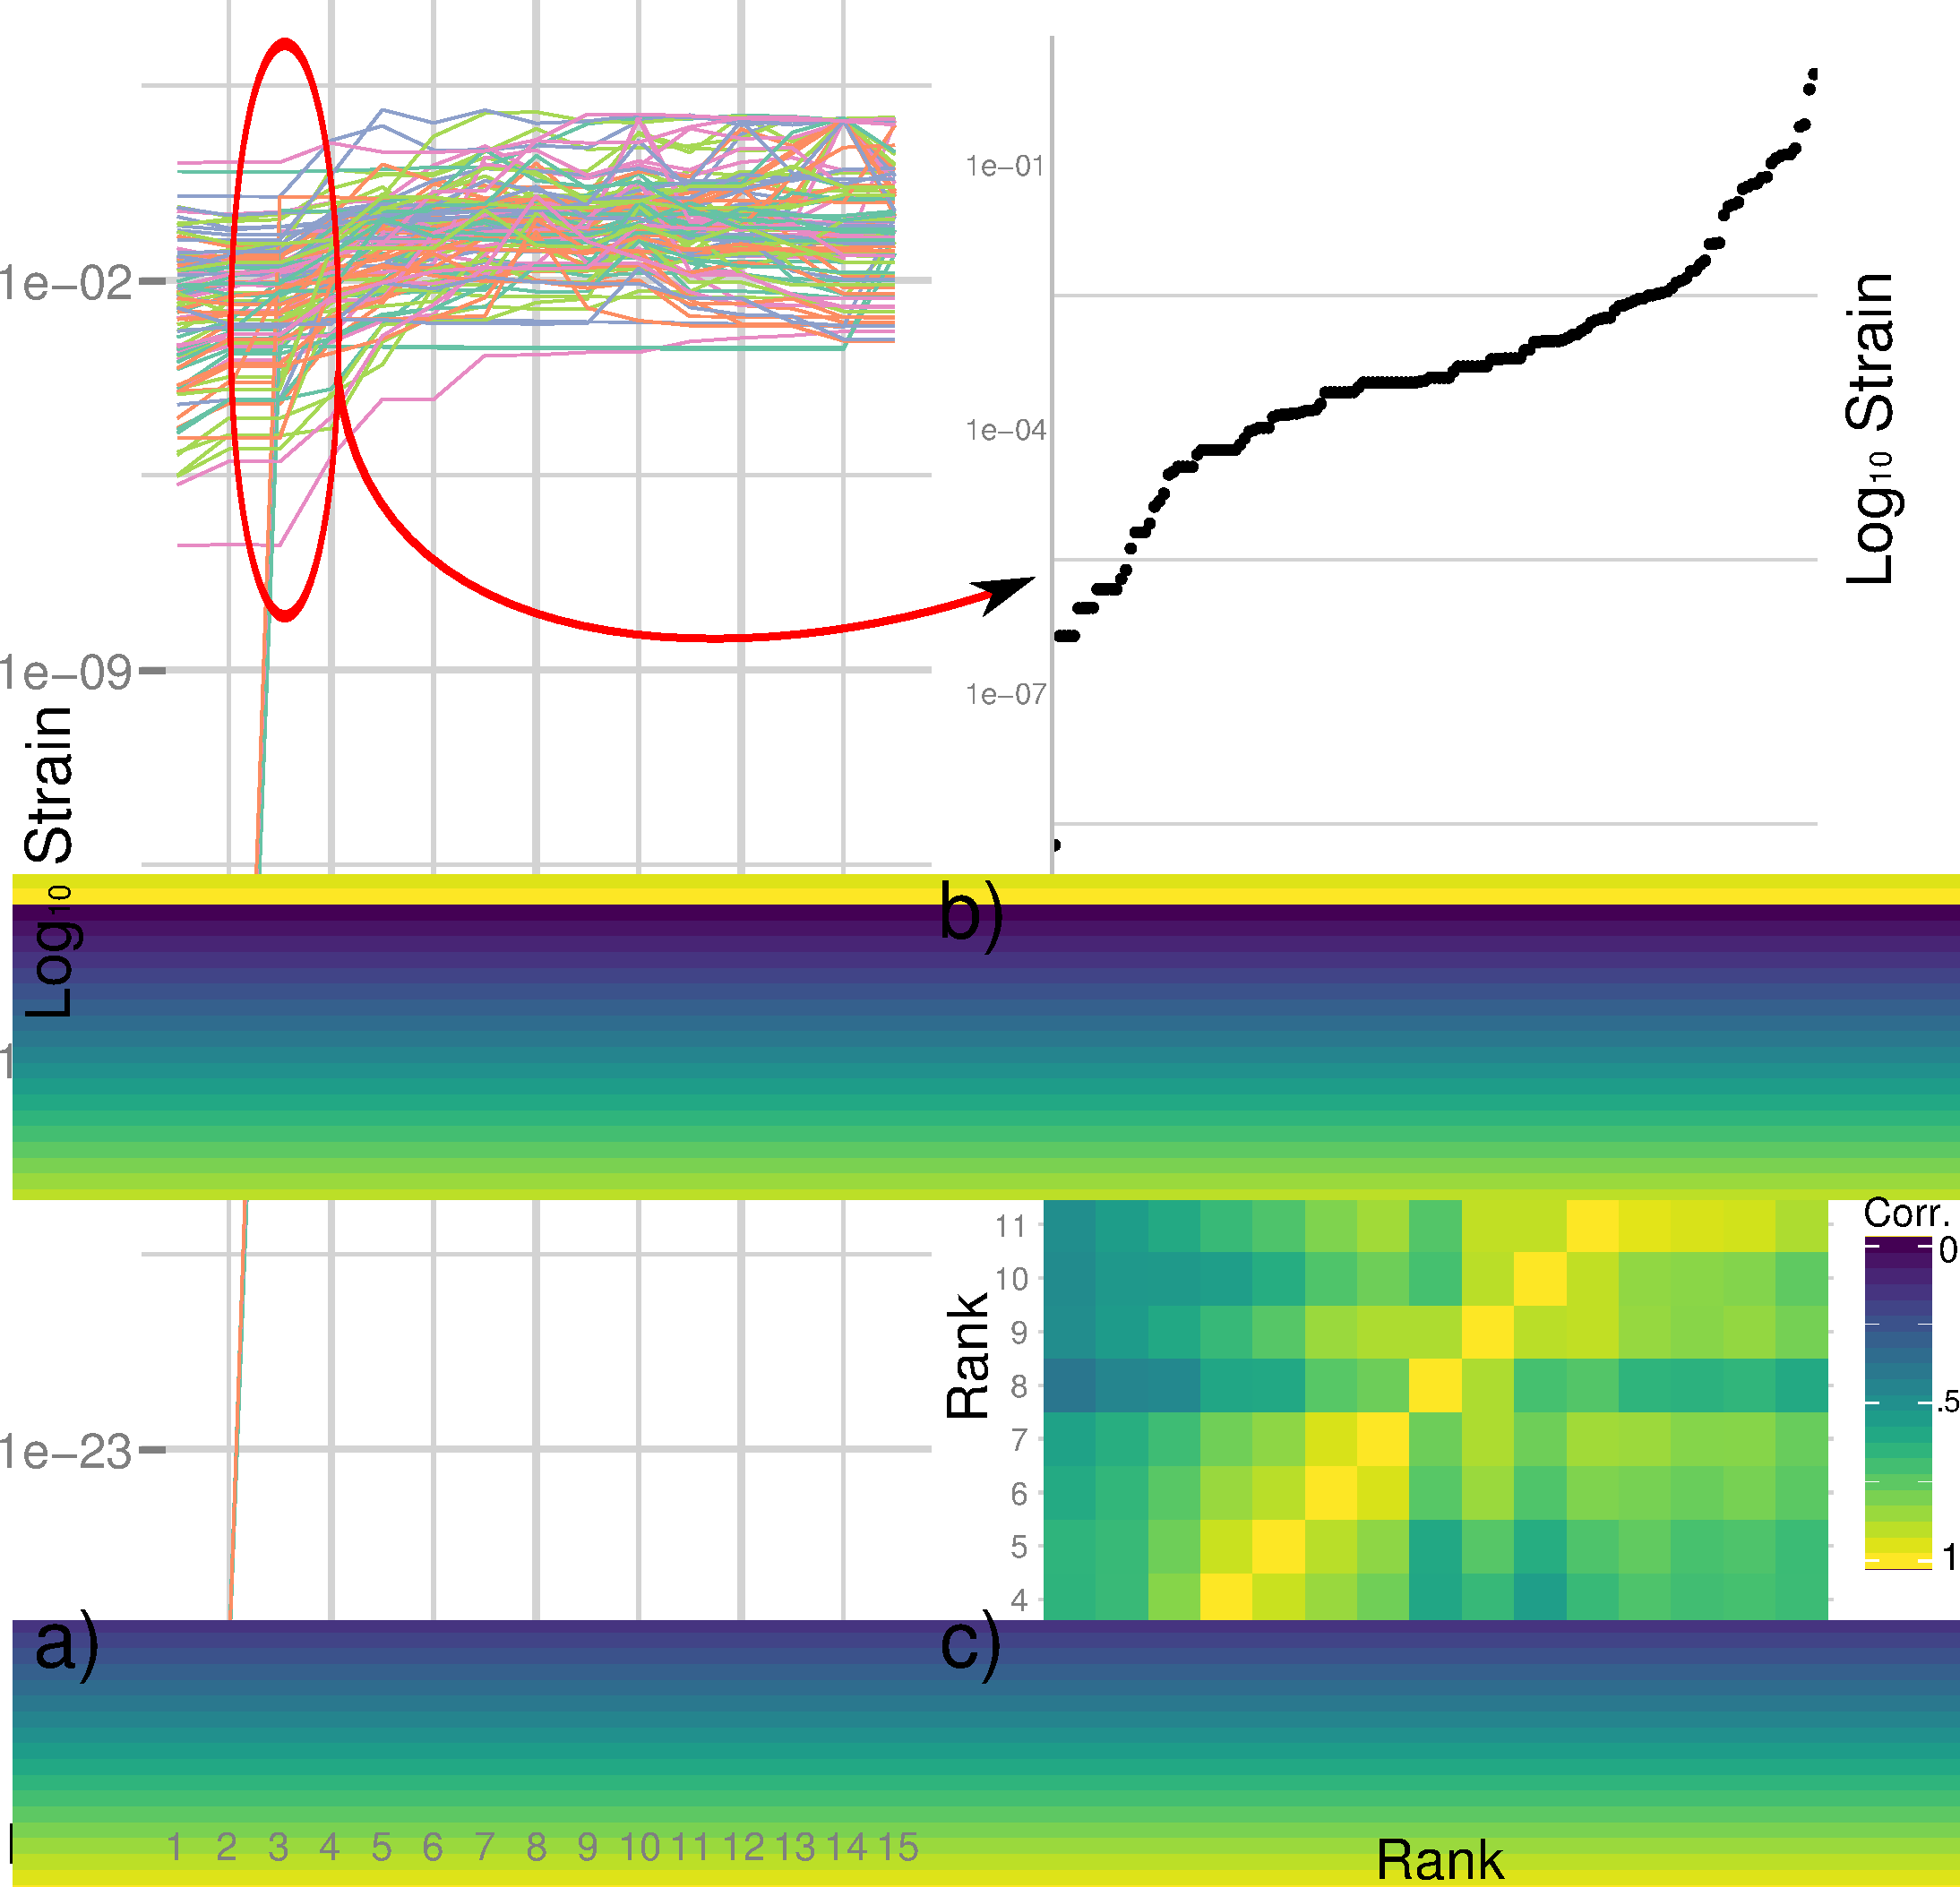
\includegraphics[width=0.7\textwidth]{./images/chap_2/Figure_1.pdf}
 \caption{The distribution of species' strain in the Serengeti National Park food web
\citep{baskerville2011spatial}.
(a) The line trace the strain of each species ($\mbox{\texttt{Log}}_{10}$ transformed) along
an increasing model dimension ($d \in \left[ 1, \dots , 15\right]$). The strain
has been computed for species as both predators and prey.
(b) A cross-section of (a) for $d  = 3$ (corresponding to the suitable model dimension).
(c) Pearson product-moment correlation coefficients for the species ordering induced by the
species' total strain across the model dimensions $d \in \left[ 1, \dots , 15\right]$.
The ordering is robust to the choice of the model dimension $d$: the Pearson's \textit{r} is consistently
above 0.5 (and all the pairwise correlations are significant at $p < 0.01$).}\label{fig:strain_1}
\end{figure}

The Afrotheria are also characterized by high uniqueness in terms of their
mean distance to the other species in the abstract functional trait space. The observation can
be extended the species' phylogeny, noticing that the two measures are non-uniformly
distributed among the tips of the phylogenetic tree (Figure~(\ref{fig:strain_2} a)). There is also support
for an Ornstein--Uhlenbeck (Brownian motion with attraction toward
an optimum) model of evolution for both strain and uniqueness (Figure~(\ref{fig:strain_2} b)).

\begin{figure}[hbt]
 \centering
 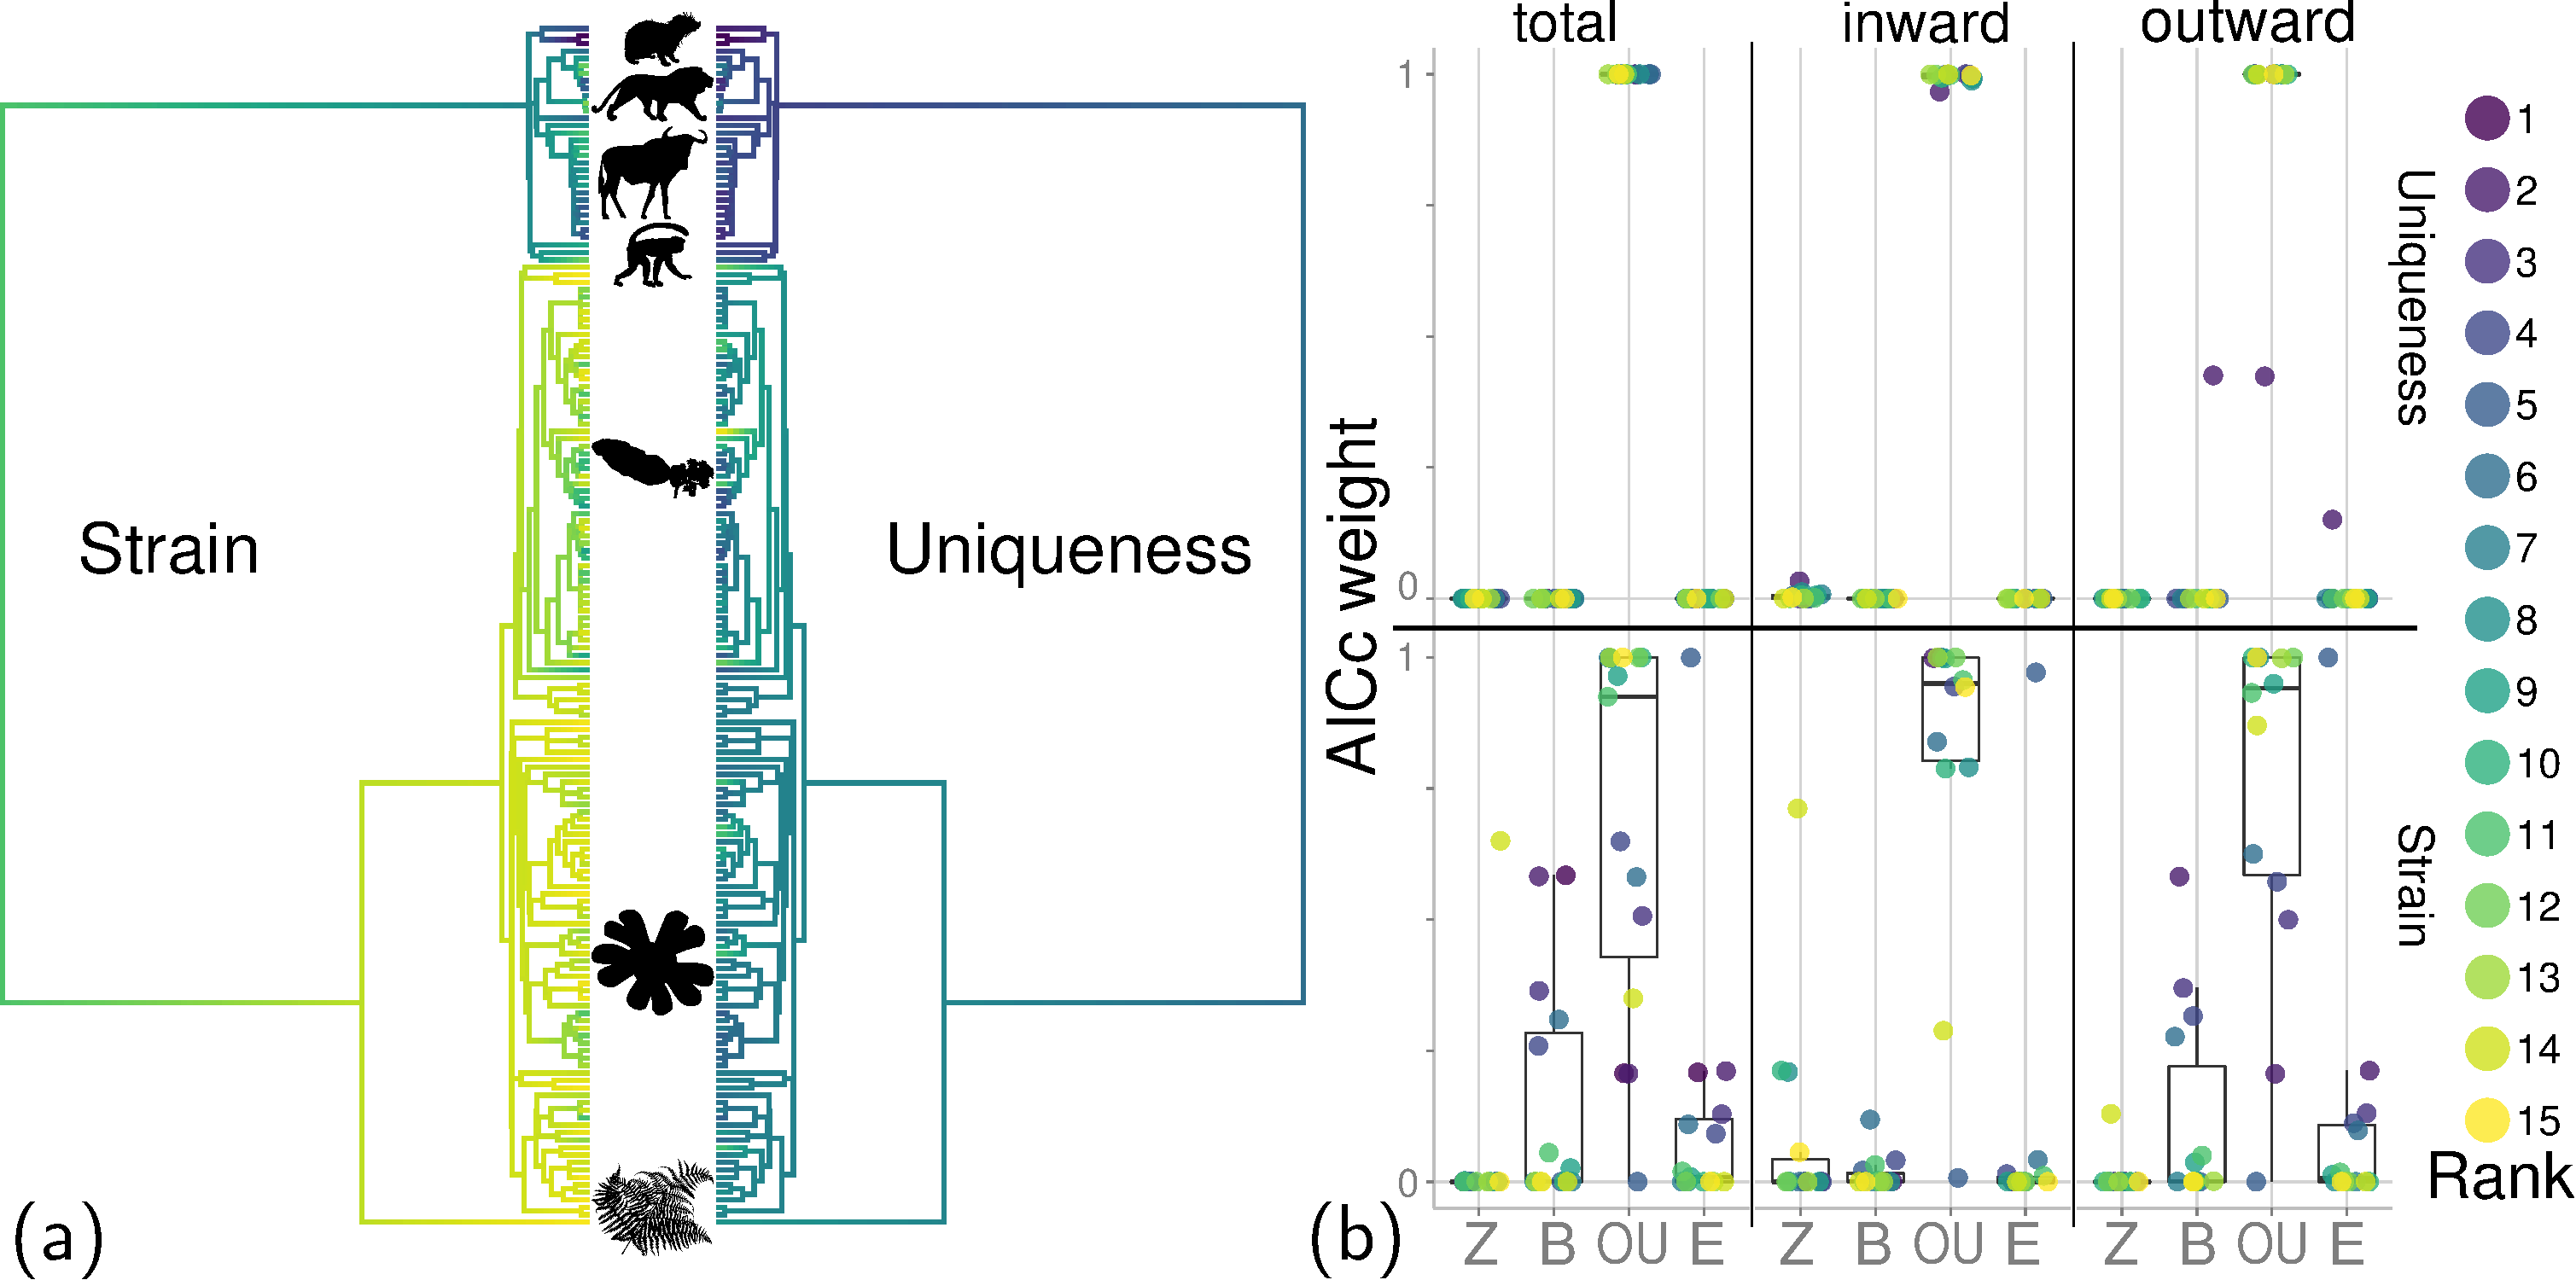
\includegraphics[width=\textwidth]{./images/chap_2/Figure_2.pdf}
 \caption{The distribution of the species' strain and uniqueness in the phylogeny
(lighter yellow for lower values; darker blue for higher values) for species as both
predators and prey (all). Here, the two measures are estimated for species as both
prey and predators and the dimension of the abstract functional traits equals 3.
The silhouettes (from phylopic.org) mark the corresponding clades:
Afrotheria (hyraxes and elephants) are the species with the highest strain and uniqueness.
(b) Akaike Information Criterion (corrected for sample size) weights for four models of species'
(inward, outward and total) strain and uniqueness evolution across the model dimensions (Rank, dark
blue for shorter functional traits, light yellow for longer functional traits):
uncorrelated, Z; Brownian motion, B \citep{felsenstein1985phylogenies};
Ornstein-Uhlenbeck, OU \citep{hansen1997stabilizing}; Early Burst, E
\citep{harmon2010early}. The data consistently supports an OU model, except
for the low-dimension strain evolution, in which there is also good support for the B model.}\label{fig:strain_2}
\end{figure}

The correlation between species' (outward and total) strain and uniqueness is
significant at $p < 0.01$, while the species' inward strain and
uniqueness are not consistently correlated for $d > 4$ (Figure~(\ref{fig:strain_3} a)). 
The computation of the species' contribution to the abstract functional
diversity for $d > 4$ (species as both predators and
prey) and $d > 7$ (species as either predators or prey) was not possible because
of software limitations. However, in the feasible range of $d$, the species' total strain is
significantly positively correlated with both the species' total uniqueness
and their contribution to the total functional diversity (Figure~(\ref{fig:strain_3} b)). The
correlations for the partial (either inward or outward) measures are not consistently
significant and depend on the measure considered.

\begin{figure}[hbt]
 \centering
 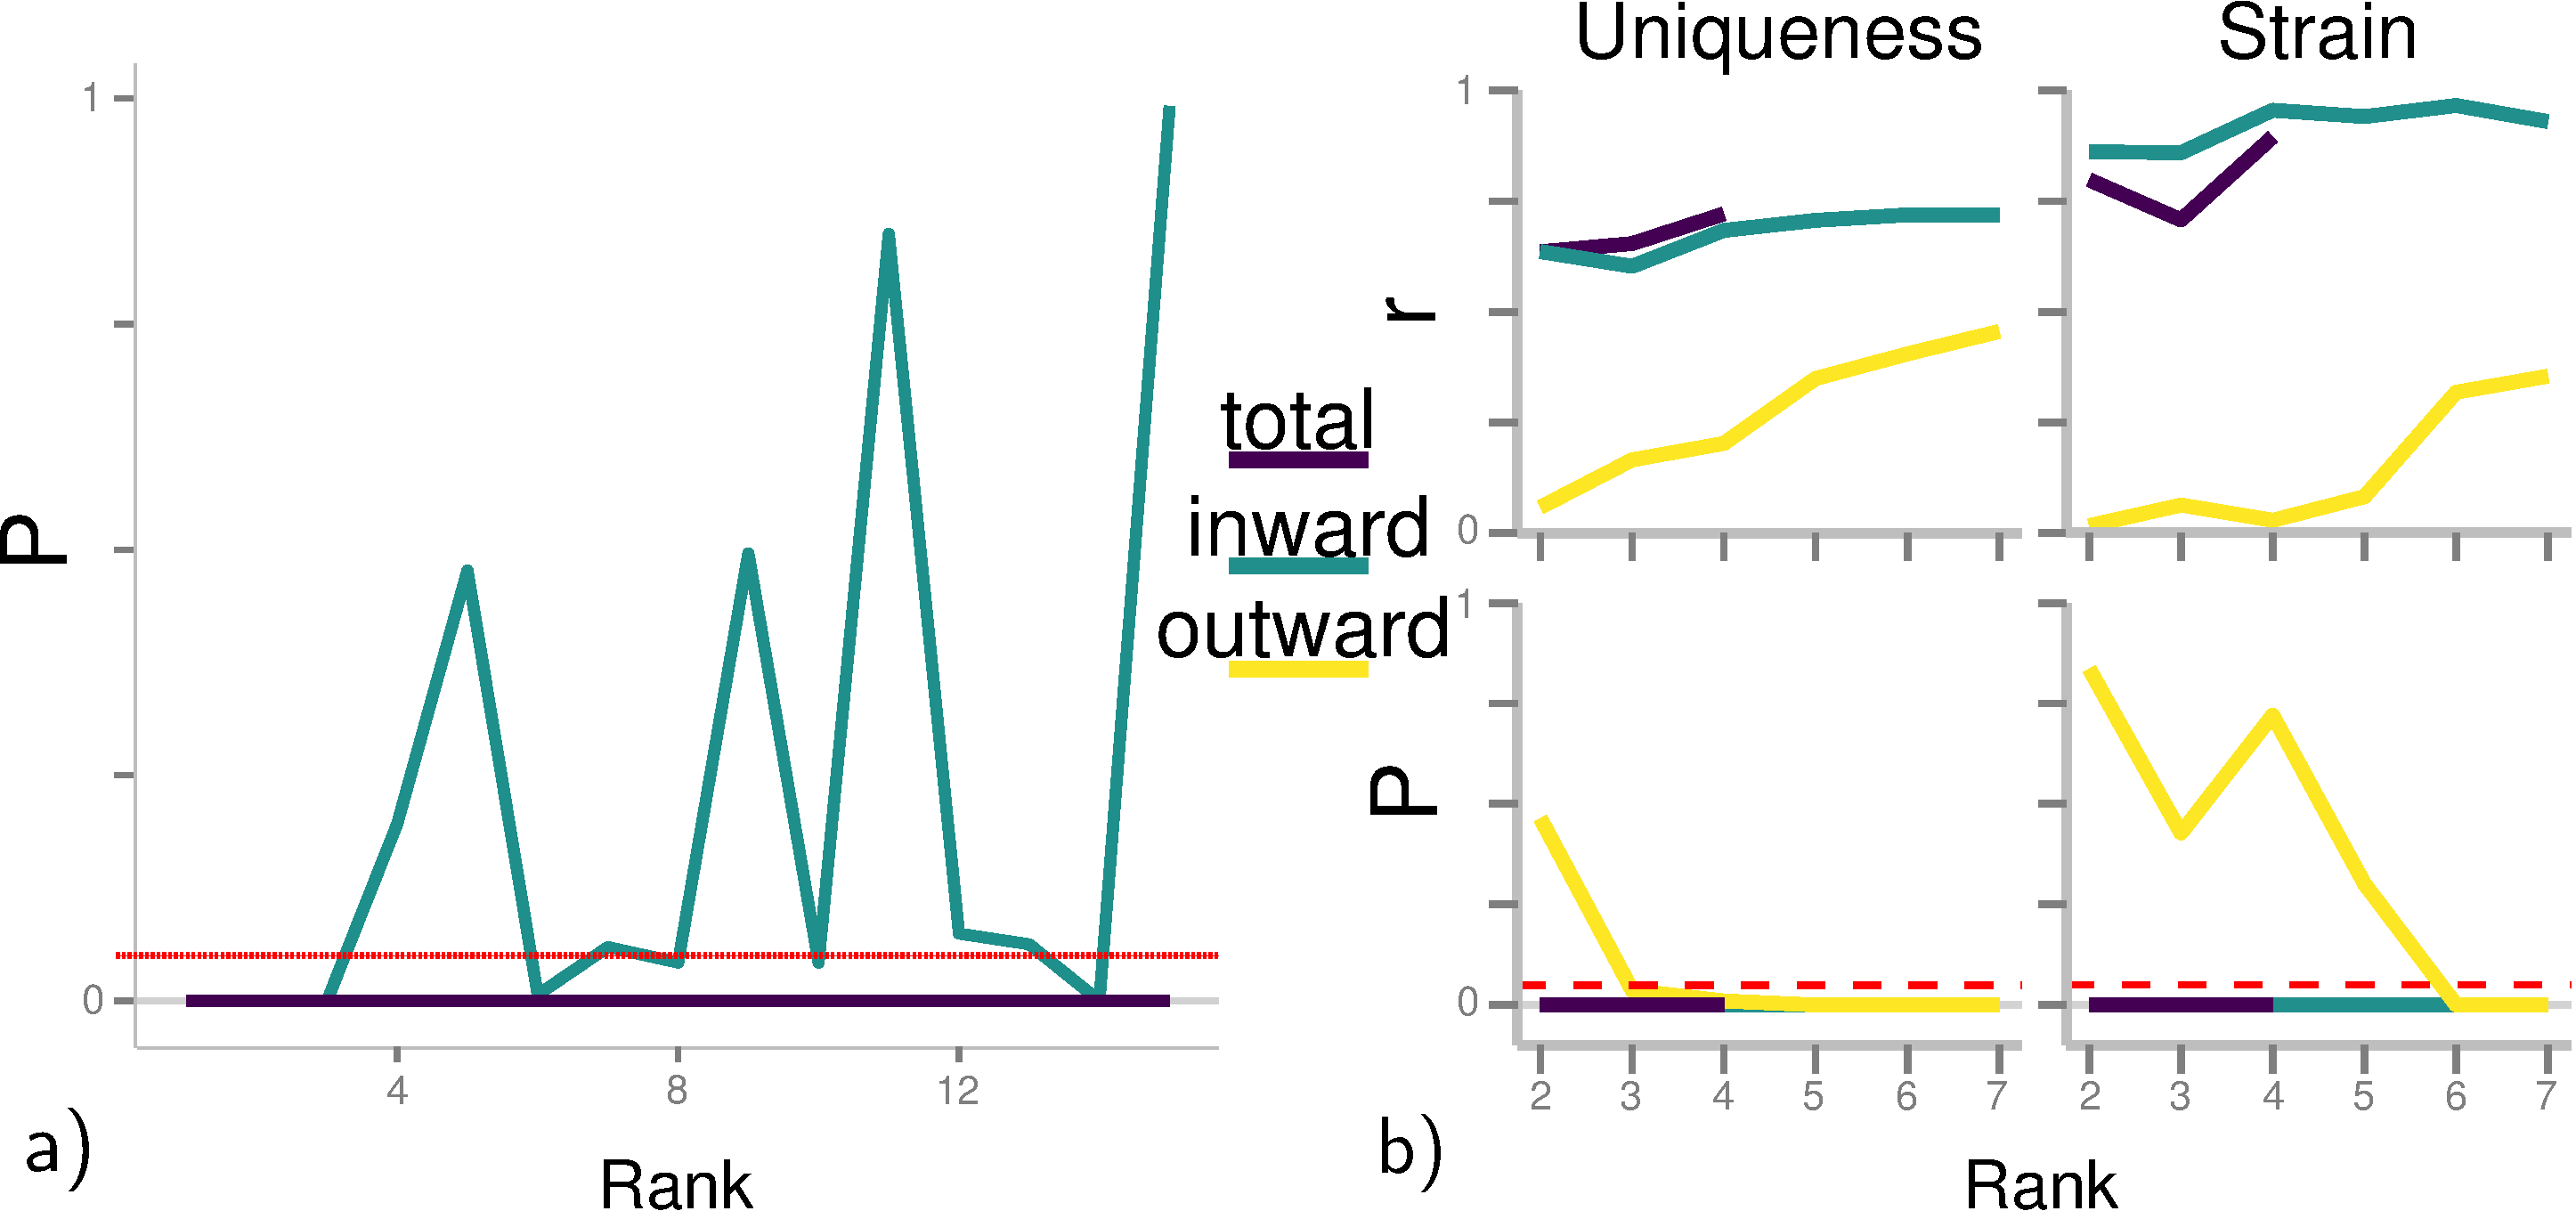
\includegraphics[width=\textwidth]{./images/chap_2/Figure_3.pdf}
 \caption{Coefficients of correlation (r) and significance (p-values, P) of a linear regression model
 of species' uniqueness and species' strain (a), and of species' contribution to functional diversity
 and species' uniqueness (b, left) and species' strain (b, right). The measures are computed
 for species as prey (inward),  for the species as a predator (outward), and for the species as predators and prey (total).
 (a) There is a significant correlation between a species' uniqueness and strain for
the species as prey (outward) and as predators and prey (total). For
model dimensions $d > 3$, the correlation is not consistently
significant for the species as a predator (inward). The yellow line (for outward traits)
is under the purple one.
(b) There is a significant correlation between the species' (inward and total) strain and
uniqueness and the species' contribution to the functional diversity (the
loss of abstract functional diversity after the removal of a species). The correlation
between a species' outward strain and contribution to functional diversity is not significant for low dimensions.
The dashed red lines correspond to $p = 0.05$.}\label{fig:strain_3}
\end{figure}

The strain and mean distance of species in the Serengeti National Park are, in
general, positively correlated with the common keystone centralities (Figure~(\ref{fig:strain_4})).
The significance and strength of the correlations depend on the particular
combination of the centrality measure, the  model dimension and the functional space
considered (either inward, outward or total). We observed the most consistent
correlations with the Betweenness, Subgraph and Degree centralities.
The correlation results are qualitatively confirmed by performing the regression analysis
either accounting for or ignoring the species' phylogenetic covariance structure. Hence
the correlations hold whether or not we consider the phylogenetic structure
of the food web. This general agreement between our novel measures and the common graph-theoretical
indices used to identify keystone species supports the applicability of the RDPG model for food
webs.

\begin{figure}[hbt]
 \centering
 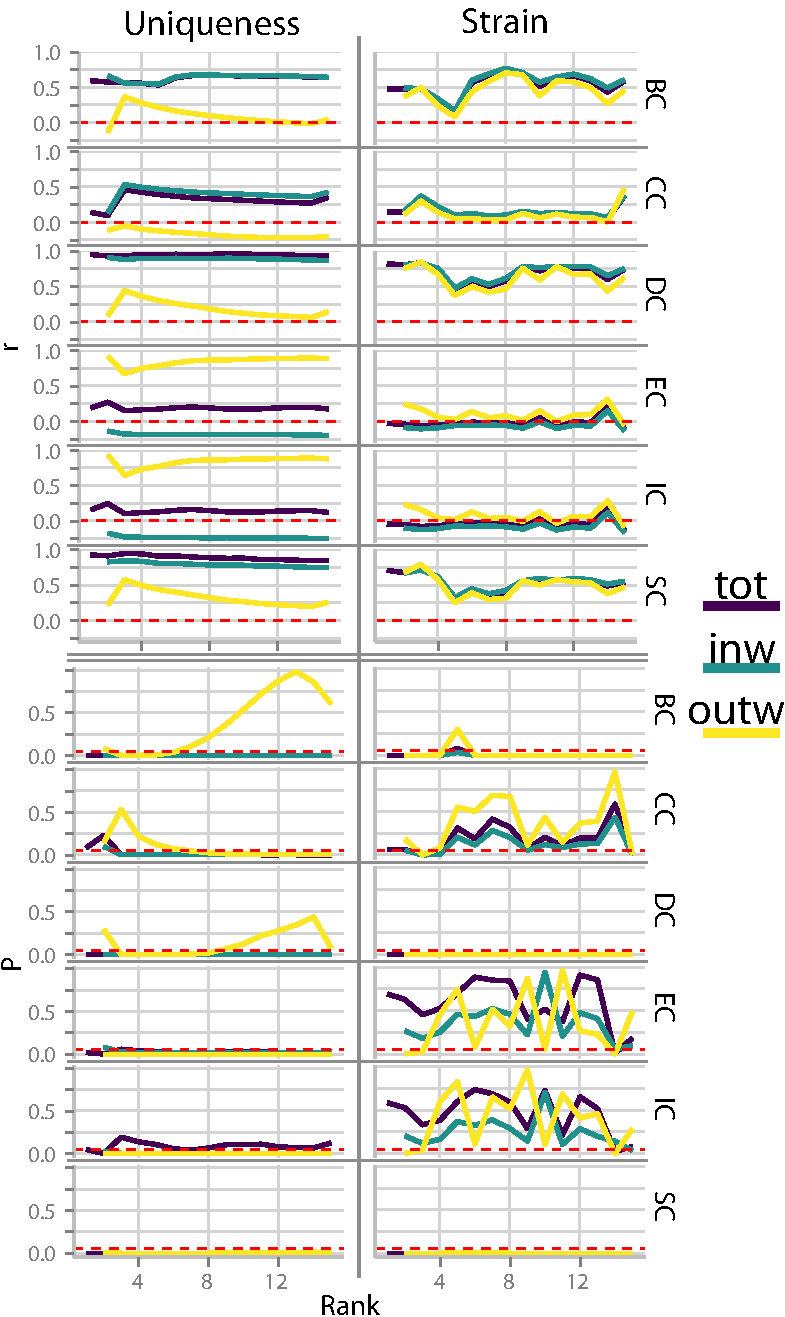
\includegraphics[height=0.6\textheight]{./images/chap_2/Figure_4.pdf}
 \caption{Coefficients of correlation (r) and significance (p-values, P) of a linear regression model
 of species' strain and uniqueness
(as a predator (inw), prey (outw) and predator and prey (tot)
and the species' betweenness (BC), closeness (CC), degree (DC),
eigenvector (EC), information (IC), and subgraph (SC)
centralities. Strengths and significances depend on the combination
of the centrality index (the correlation is significant for most centralities
except EC and IC), functional space (the correlation with the outward strain
and uniqueness is weak) and model dimension (the correlation is stronger
for low $d$). The dashed red lines correspond to $r = 0$ and $p = 0.05$. Notice that when more than
one of the species' measures as a predator, prey or predator and prey are significant, they line overlap
and hide each other.}\label{fig:strain_4}
\end{figure}

Although there are species with both high phylogenetic distinctiveness and high
strain or uniqueness (Table~(\ref{tab:strain_1})), we did not detect any significant linear
correlation between the species' evolutionary and ecological relevance measures.

\begin {table}[hbt]
\begin{tabular}{|l|*{4}{c|}}
\hline
Species	&Strain	&Uniqueness	&Diversity &Equal Splits\\
\hline
\emph{Procavia capensis}	&1.32	&1	&3	&6.5\\
\emph{Heterohyrax brucei}	&0.88	&2	&1	&6.5\\
\emph{Loxodonta africana}	&0.32	&7	&6	&2\\
\emph{Panthera pardus}		&0.31	&3	&10	&148.5\\
\emph{Panthera leo}		&0.18	&6	&4	&148.5\\
\emph{Eudorcas thomsonii}	&0.17	&8	&19	&150.5\\
\emph{Nanger granti}		&0.16	&5	&13	&150.5\\
\emph{Connochaetes taurinus}	&0.15	&4	&14	&138\\
\emph{Madoqua kirkii}		&0.15	&11	&2	&100\\
\emph{Aepyceros melampus}	&0.12	&13	&0	&100\\
\hline
\end{tabular}
\caption{The 10 species in the Serengeti National Park food web
\citep{baskerville2011spatial} with the highest strain (as both predators and prey)
and their ordering based on ecological uniqueness  (as both predators and
prey), contribution to functional diversity (diversity, as both predators and
prey) and equal splits (a measure of evolutionary distinctiveness). Strain,
uniqueness and contribution to functional diversity are positively correlated.
However, although there are species (e.g., the Afrotheria clade) with a high
score in all four measures, in general, there is no significant linear correlation between
ecological relevance and evolutionary distinctiveness.}\label{tab:strain_1}
\end{table}

Finally, the correlation between the topological and the (simulated) weighted rankings are
significant and positive for more than $95\%$ of the simulations. However, the amount of variation in the weighted
ranking explained by the topological ranking varies (i.e., it spans the range from almost null
to almost one). Yet, the set of species with higher \emph{strain} and the set of species with higher \emph{mean distance}
as estimated from the topological data was consistent across the simulated weighted networks, indicating
that our measures are able to identigy the species with distinctively high ecological importance (see Supplementary Material).

 \section{Discussion}

For each species in the food web, we estimated its position in the (inward, outward and
total) abstract functional trait space for $d \in \left[ 1, \dots, 15\right]$
and computed three measures of ecological relevance (strain, uniqueness and
contribution to functional diversity). We verified that species' ordering
based on the measures we introduced is robust to the choice of the model's dimension
$d$. The RDPG model for food webs allows us to distinguish between the low-dimensional,
stochastic backbone of a food web and its fine wiring. The
stochastic backbone is robust to food web variability and to misspecifications
of the food web structure, such as a missed observation of an interaction or
an erroneous recording.  Being based on the estimated (low-dimensional)
structural food-web backbone, the measures we introduced are themselves robust
to the variability of complex food webs. Other classic measures of trophic
uniqueness \citep{yodzis1999search,luczkovich2003defining,jordan2009trophic} do
not make this distinction.

The RDPG model allows us to estimate the abstract functional
diversity of a food web by relying solely on topological data. 
It remains to be ascertained whether there is a correspondence between the classic
morphological functional diversity and our novel concept of abstract
functional diversity. If verified, the abstract functional diversity may serve
to estimate the (classic) functional diversity without the burden of
identifying suitable phenotypic traits with a functional role across all the
species in a food web---an ambitious task, given species' heterogeneity. 
Our results point toward a positive answer. The
range of suitable abstract space dimensions estimated under the RDPG model,
is in good accordance with the number of (classic) functional traits that \citet{maire2015many}
estimated for an optimal (classic) functional diversity analysis.

\citet{petchey2008trophically} have shown that trophically unique species
are exposed to a higher risk of secondary extinction; in addition, \citet{o2010loss} provided evidence that
food webs are particularly fragile to the extinction of functionally unique species.
Our results indicate that a species' strain  is positively correlated with  the mean distance of that
species to the other species in the (inward, outward or total) functional trait space;
in other words, the ecological uniqueness of a species is  a good predictor of the magnitude of the effect
of its extinction. Moreover, both strain and uniqueness are positively correlated
with a species' contribution to the abstract functional diversity of the food
web. The results appear robust across binary and weighted version of the food webs:
the ranking of the species based on strain and uniqueness as computed from (simulated) weighted food webs
were consistently predicted by the ranking computed from the corresponding binary food webs.

We showed that a species' abstract functional trait uniqueness and its strain are both positively
correlated with its classic centrality in the Serengeti National Park food web.
The result was also confirmed for the Weddell Sea food web
\citep{jennings2002long}, the Caribbean Sea food web \citep{opitz1996trophic}
and the independent compilation of the Serengeti National Park food web by \citet{de2011serengeti}
supporting the notion that the methodology here introduced can be used on different
systems. A positive correlation between classic functional uniqueness, \emph{sensu}
\citet{yodzis1999search},  and the degree centrality---the number of trophic
interactions, which is one of the classic centrality we consider---has already
been observed by \citet{petchey2008trophically}.  The
result is even more interesting if read in comparison with the negative
correlation found by \citet{lai2012centrality} between the classic centralities
and the trophic uniqueness of a species \emph{sensu} \citet{luczkovich2003defining}
and \citet{jordan2009trophic}. Our results, here, suggest that uniqueness (mean distance)
and centrality (strain) are indeed positively correlated (and, thus, appear to confirm  \citet{petchey2008trophically}'s
observation). However, further comparative analyses are
needed to explain this difference and explore the relationship between the abstract
functional uniqueness of a species and its trophic uniqueness as otherwise
defined. Yet to be fully explained are also the precise relation between RDPG centralities
and classic (topological) centralities: indeed, the behaviour of the correlations between the
various measures appear to depend, in the details, on the considered food web, although
the general trends are observed in all the webs.

The ecological relevance---strain and uniqueness---of the species in the Serengeti food web
is not uniformly distributed across the phylogeny (in fact, it is compatible with the distribution
we would expect under a Ornstein-Uhlenbeck model of evolution \citep{hansen1997stabilizing}). We did not detect a
significant correlation between the species' ecological relevance and their
evolutionary distinctiveness. However, a small number of species have both
high ecological relevance and high evolutionary distinctiveness. This is the
case in the Afrotheria clade (i.e., the African elephants and two hyrax species).
The peculiarity of the Afrotheria clade has already been suggested by \citet{baskerville2011spatial}
on the basis of the particularity of the hyrax's trophic role.
Our results confirms the importance of considering both ecological and evolutionary factors
in the evaluation of species for conservation purposes.

%%%%%%%%%% Insert bibliography here %%%%%%%%%%%%%%
\small
\singlespacing
\bibliography{DallaRiva_RSOS.bib}

\end{document}
